\documentclass[12pt,a4paper]{article}
\usepackage[utf8]{inputenc}
\usepackage[margin=3cm]{geometry} % margins
%\linespread{1.2} % line spacing
\usepackage{graphicx} % Required for inserting images
\usepackage{hyperref}
\usepackage{subcaption}
\usepackage{float}
\usepackage{tcolorbox}
\usepackage{amsmath}
\usepackage{amssymb}
\usepackage{listings}% http://ctan.org/pkg/listings}
\usepackage{algorithm}
\usepackage{algorithmic}
\usepackage[toc,page]{appendix}
\usepackage{multicol}
\usepackage{siunitx}
\usepackage{comment}
\usepackage{xcolor}
\usepackage{caption}
\usepackage{forest}
\usepackage{tikz}
\usetikzlibrary{shapes.geometric, arrows}
\usepackage{todonotes} %\setuptodonotes{tickmarkheight=4pt}

\newtheorem{definition}{Definition}

\tikzstyle{startstop} = [rectangle, rounded corners, 
minimum width=3cm, 
minimum height=1cm,
text centered, 
draw=black, 
fill=red!30]

\tikzstyle{io} = [trapezium, 
trapezium stretches=true, % A later addition
trapezium left angle=70, 
trapezium right angle=110, 
minimum width=3cm, 
minimum height=1cm, text centered, 
draw=black, fill=blue!30]

\tikzstyle{process} = [rectangle, 
minimum width=3cm, 
minimum height=1cm, 
text centered, 
text width=3cm, 
draw=black, 
fill=orange!30]

\tikzstyle{decision} = [diamond, 
minimum width=3cm, 
minimum height=1cm, 
text centered, 
draw=black, 
fill=green!30]
\tikzstyle{arrow} = [thick,->,>=stealth]

% To delete lstlisting caption "Listing x"
%\captionsetup[lstlisting]{labelformat=empty}

\lstdefinestyle{myStyle}{
    belowcaptionskip=1\baselineskip,
    breaklines=true,
    frame=none,
    numbers=none, 
    basicstyle=\footnotesize\ttfamily,
    keywordstyle=\bfseries\color{green!40!black},
    commentstyle=\itshape\color{purple!40!black},
    identifierstyle=\color{black},
    backgroundcolor=\color{white},
}

\lstdefinestyle{csvStyle}{
    basicstyle=\ttfamily\small, % Use a typewriter font
    columns=fullflexible, % Better column alignment
    %frame=single, % Add a border
    %backgroundcolor=\color{gray!10}, % Light gray background
    keywordstyle=\color{blue}\bfseries, % Style for keywords (optional)
    morekeywords={name,code,loc_latitude,loc_longitude, ATM_id, city, country,
    number_id, client_id, expiration, CVC, extract_limit, amount_avg_withdrawal,amount_std_withdrawal,withdrawal_day,
    amount_avg_deposit,amount_std_deposit,deposit_day,inquiry_day,
    amount_avg_transfer,amount_std_transfer,transfer_day,
    transaction_id,number_id,ATM_id,transaction_type,transaction_start,
    transaction_end, transaction_amount}, % Highlight CSV headers as keywords
    showstringspaces=false,
    captionpos=b,                    % sets the caption-position to bottom
}

\lstdefinestyle{cypherStyle}{
    backgroundcolor=\color{white},   % choose the background color
    basicstyle=\footnotesize\ttfamily,        % the size of the fonts that are used for the code
    commentstyle=\itshape\color{purple!40!black},
    keywordstyle=\bfseries\color{green!40!black},
    breakatwhitespace=false,         % sets if automatic breaks should only happen at whitespace
    breaklines=true,                 % sets automatic line breaking
    captionpos=b,                    % sets the caption-position to bottom
    commentstyle=\color{gray},    % comment style
    deletekeywords={},            % if you want to delete keywords from the given language
    escapeinside={\%*}{*)},          % if you want to add LaTeX within your code
    extendedchars=true,              % lets you use non-ASCII characters; for 8-bits encodings only, does not work with UTF-8
    %firstnumber=1000,                % start line enumeration with line 1000
    frame=none,                    % adds a frame around the code
    keepspaces=true,                 % keeps spaces in text, useful for keeping indentation of code (possibly needs columns=flexible)
    language=SQL,                    % the language of the code
    morekeywords={*,IF, REQUIRE, FOR, IS, LOAD, CSV, WITH, HEADERS, MERGE, toFloat, toInteger, date},            % if you want to add more keywords to the set
    numbers=none,                    % where to put the line-numbers; possible values are (none, left, right)
    numbersep=5pt,                   % how far the line-numbers are from the code
    numberstyle=\tiny\color{mygray}, % the style that is used for the line-numbers
    rulecolor=\color{black},         % if not set, the frame-color may be changed on line-breaks within not-black text (e.g. comments (green here))
    showspaces=false,                % show spaces everywhere adding particular underscores; it overrides 'showstringspaces'
    showstringspaces=false,          % underline spaces within strings only
    showtabs=false,                  % show tabs within strings adding particular underscores
    stepnumber=1,                    % the step between two line-numbers. If it's 1, each line will be numbered
    stringstyle=\ttfamily,     % string literal style
    tabsize=2,                       % sets default tabsize to 2 spaces
}

%% Golang definition for listings
%% http://github.io/julienc91/lstlistings-golang
%%
\lstdefinelanguage{Golang}%
  {morekeywords=[1]{package,import,func,type,struct,return,defer,panic,%
     recover,select,var,const,iota,},%
   morekeywords=[2]{string,uint,uint8,uint16,uint32,uint64,int,int8,int16,%
     int32,int64,bool,float32,float64,complex64,complex128,byte,rune,uintptr,%
     error,interface},%
   morekeywords=[3]{map,slice,make,new,nil,len,cap,copy,close,true,false,%
     delete,append,real,imag,complex,chan,},%
   morekeywords=[4]{for,break,continue,range,go,goto,switch,case,fallthrough,if,%
     else,default,},%
   morekeywords=[5]{Println,Printf,Error,Print,},%
   sensitive=true,%
   morecomment=[l]{//},%
   morecomment=[s]{/*}{*/},%
   morestring=[b]',%
   morestring=[b]",%
   morestring=[s]{`}{`},%
}

\lstdefinestyle{golangStyle}{
    captionpos=b,              % sets the caption-position to bottom
    belowcaptionskip=1\baselineskip,
    breaklines=true,
    frame=none,
    numbers=none, 
    basicstyle=\footnotesize\ttfamily,
    keywordstyle=\bfseries\color{green!40!black},
    commentstyle=\scriptsize\itshape\color{gray},
    identifierstyle=\color{black},
    backgroundcolor=\color{white},
    language=Golang,
    tabsize=1,                 % reduces the tab size (number of spaces per tab)
    keepspaces=true,           % preserves spaces and tabs exactly as written
    showspaces=false,          % hides visible spaces
    showtabs=false             % hides visible tabs
}

\setlength{\parindent}{0pt} % QUITAR SANGRÍAS
\captionsetup{font=small} % Fuente del texto de las imagenes

\newcommand{\DP}{$\mathsf{DP}$ }
\newcommand{\DPATM}{$\mathsf{DP_{ATM}}$ }

\newcommand{\alertch}{$\mathsf{alert}$ }
\newcommand{\eventch}{$\mathsf{event}$ }
\newcommand{\internaledgech}{$\mathsf{internal\_edge}$ }

\newcommand{\cardsubgraph}{$\mathsf{cs}$ }

\newcommand{\filter}{\emph{Filter} }
\newcommand{\source}{\emph{Source} }
\newcommand{\sink}{\emph{Sink} }
\newcommand{\generator}{\emph{Generator} }
\newcommand{\filterworker}{\emph{Filter Worker} }

\newcommand{\F}{$\mathsf{F}$ }
\newcommand{\Sr}{$\mathsf{Sr}$ }
\newcommand{\Sk}{$\mathsf{Sk}$ }
\newcommand{\G}{$\mathsf{G}$ }
\newcommand{\FW}{$\mathsf{FW}$ }

\newenvironment{graysection}
  {\begingroup\color{gray}} % Start with gray color
  {\endgroup}               % End the color group

%%%%%%%
\newcommand{\ep}[1]{\todo[inline,backgroundcolor=orange!70,textcolor=black]{\tiny \textbf{Edelmira:} #1}}
%%%%%%
%%%%%%%
\newcommand{\fmc}[1]{\todo[inline,backgroundcolor=blue!40,textcolor=black]{\small \textbf{Fernando:} #1}}
%%%%%%

%%%%%%%
\newcommand{\ad}[1]{\todo[inline,backgroundcolor=green!40,textcolor=black]{\tiny \textbf{Amalia:} #1}}
%%%%%%

\title{TFM-FernandoMartín}
\author{Fernando Martín Canfrán}
\date{\today}

\begin{document}

\maketitle

\section{Analysis of Results}

Objectives to answer:
\begin{itemize}
    \item How does it behave the \DPATM. Is it worthy wrt to a sequential / non-multiple filter
    version?
\end{itemize}

\subsection{Small GDB}

Note: 1f is the equivalent sequential version... in these experiments.

\subsubsection{For each stream size}

1. How the different configurations behave - 

\paragraph{Radial plots - for each stream - comparing among the different number of cores configurations\\}
\newpage

\begin{figure}[H]
    \centering
    % Temporarily adjust margins for wider content
    \makebox[\textwidth][c]{%
        \begin{minipage}{0.5\textwidth}
            \centering
            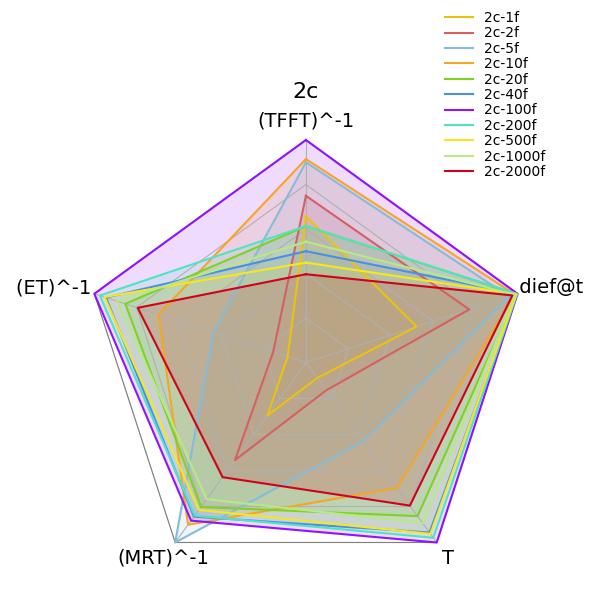
\includegraphics[scale=0.6]{../processed/NRT/small/checks/30-0.02/fixedcores/2c/plots/radar-dieft.png}
            \caption*{}
        \end{minipage}
        \hspace{0.08\textwidth}
        \begin{minipage}{0.5\textwidth}
            \centering
            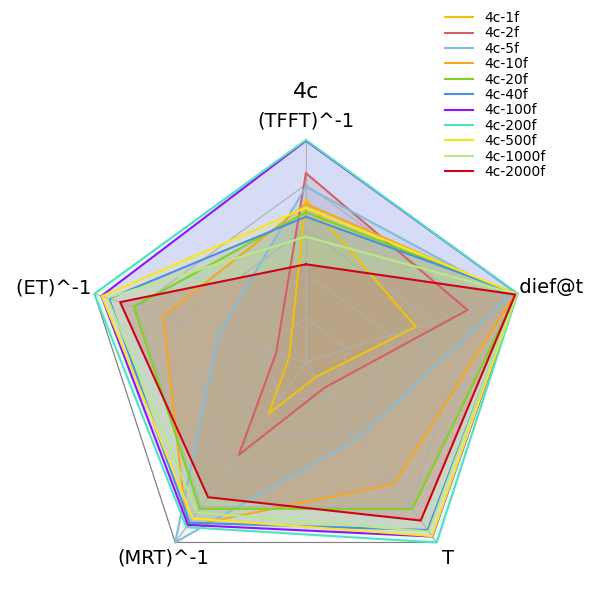
\includegraphics[scale=0.6]{../processed/NRT/small/checks/30-0.02/fixedcores/4c/plots/radar-dieft.png}
            \caption*{}
        \end{minipage}
    }
    
    \vspace{0.5cm} % Vertical space between rows

    \makebox[\textwidth][c]{%
        \begin{minipage}{0.5\textwidth}
            \centering
            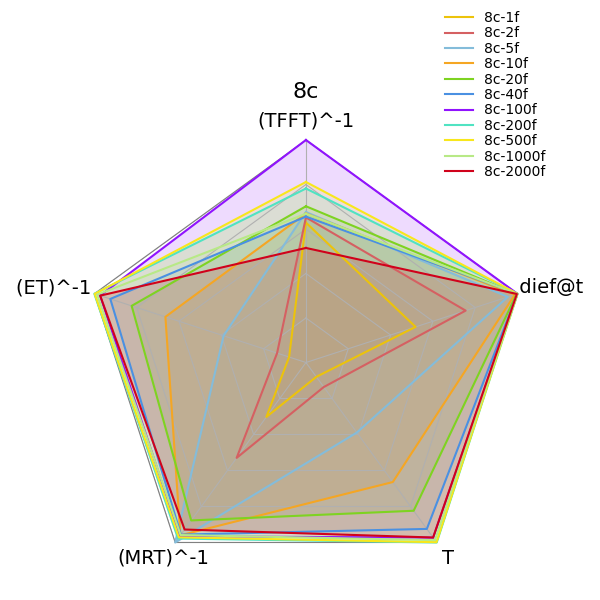
\includegraphics[scale=0.6]{../processed/NRT/small/checks/30-0.02/fixedcores/8c/plots/radar-dieft.png}
            \caption*{}
        \end{minipage}
        \hspace{0.08\textwidth}
        \begin{minipage}{0.5\textwidth}
            \centering
            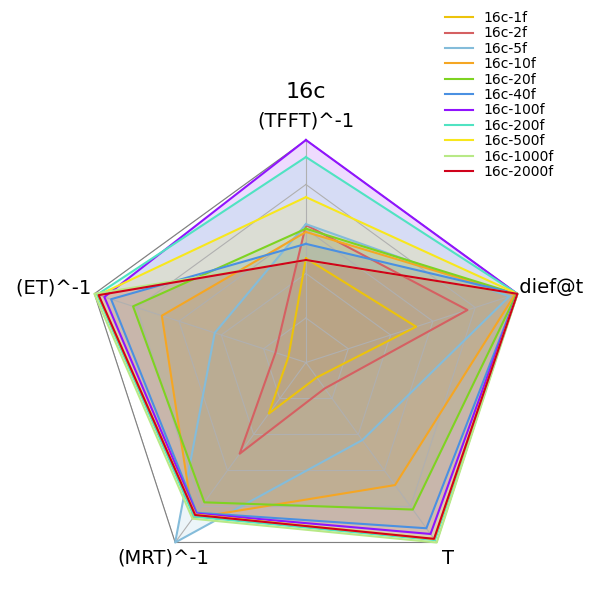
\includegraphics[scale=0.6]{../processed/NRT/small/checks/30-0.02/fixedcores/16c/plots/radar-dieft.png}
            \caption*{}
        \end{minipage}
    }

    \caption{Radial Plots for small stream: 30-0.02}
    \label{img:exps-read-input-variants}
\end{figure}

\begin{figure}[H]
    \centering
    % Temporarily adjust margins for wider content
    \makebox[\textwidth][c]{%
        \begin{minipage}{0.5\textwidth}
            \centering
            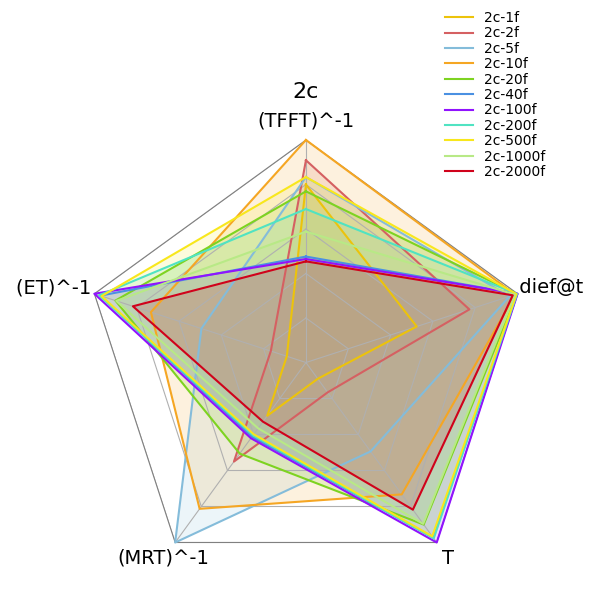
\includegraphics[scale=0.6]{../processed/NRT/small/checks/60-0.02/fixedcores/2c/plots/radar-dieft.png}
            \caption*{}
        \end{minipage}
        \hspace{0.08\textwidth}
        \begin{minipage}{0.5\textwidth}
            \centering
            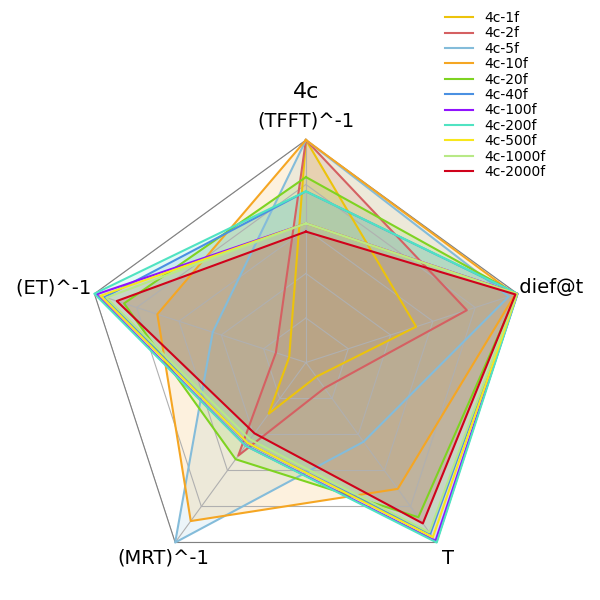
\includegraphics[scale=0.6]{../processed/NRT/small/checks/60-0.02/fixedcores/4c/plots/radar-dieft.png}
            \caption*{}
        \end{minipage}
    }
    
    \vspace{0.5cm} % Vertical space between rows

    \makebox[\textwidth][c]{%
        \begin{minipage}{0.5\textwidth}
            \centering
            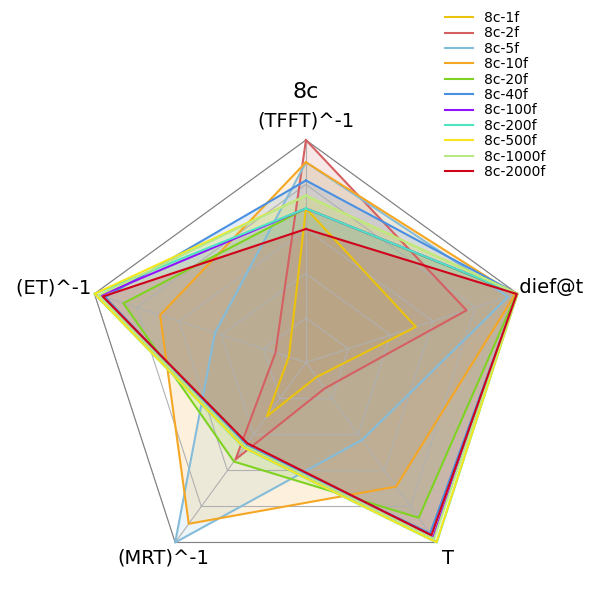
\includegraphics[scale=0.6]{../processed/NRT/small/checks/60-0.02/fixedcores/8c/plots/radar-dieft.png}
            \caption*{}
        \end{minipage}
        \hspace{0.08\textwidth}
        \begin{minipage}{0.5\textwidth}
            \centering
            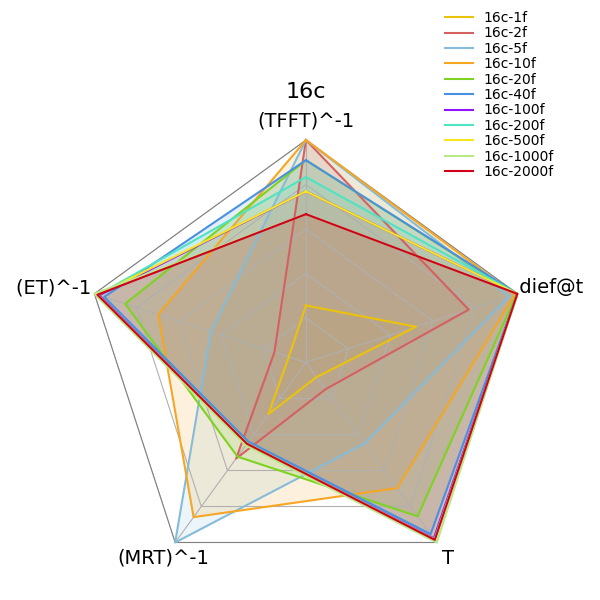
\includegraphics[scale=0.6]{../processed/NRT/small/checks/60-0.02/fixedcores/16c/plots/radar-dieft.png}
            \caption*{}
        \end{minipage}
    }

    \caption{Radial Plots for medium stream: 60-0.02}
    \label{img:exps-read-input-variants}
\end{figure}

\begin{figure}[H]
    \centering
    % Temporarily adjust margins for wider content
    \makebox[\textwidth][c]{%
        \begin{minipage}{0.5\textwidth}
            \centering
            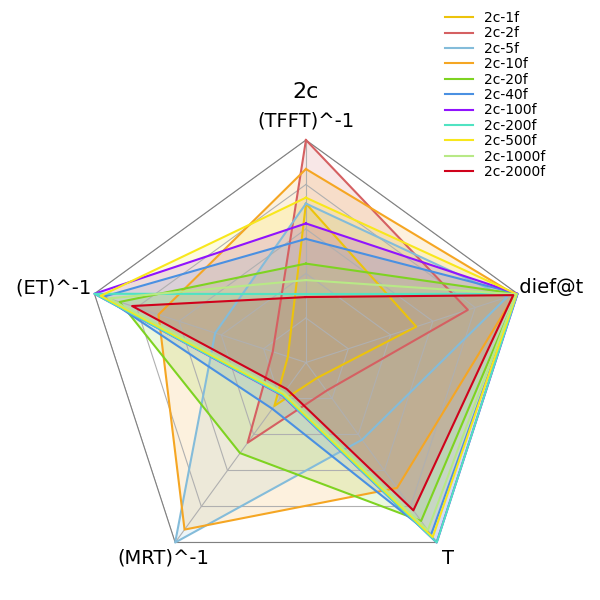
\includegraphics[scale=0.6]{../processed/NRT/small/checks/120-0.02/fixedcores/2c/plots/radar-dieft.png}
            \caption*{}
        \end{minipage}
        \hspace{0.08\textwidth}
        \begin{minipage}{0.5\textwidth}
            \centering
            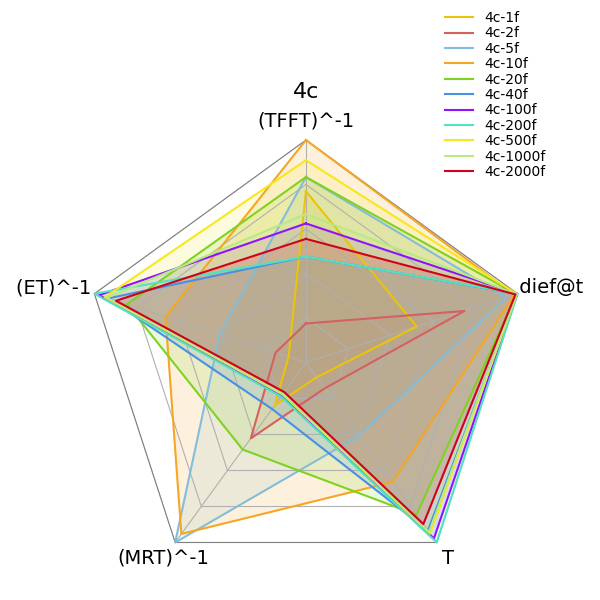
\includegraphics[scale=0.6]{../processed/NRT/small/checks/120-0.02/fixedcores/4c/plots/radar-dieft.png}
            \caption*{}
        \end{minipage}
    }
    
    \vspace{0.5cm} % Vertical space between rows

    \makebox[\textwidth][c]{%
        \begin{minipage}{0.5\textwidth}
            \centering
            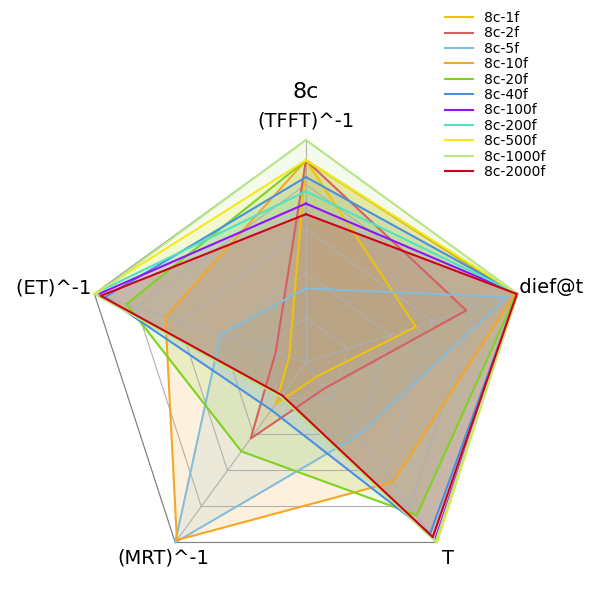
\includegraphics[scale=0.6]{../processed/NRT/small/checks/120-0.02/fixedcores/8c/plots/radar-dieft.png}
            \caption*{}
        \end{minipage}
        \hspace{0.08\textwidth}
        \begin{minipage}{0.5\textwidth}
            \centering
            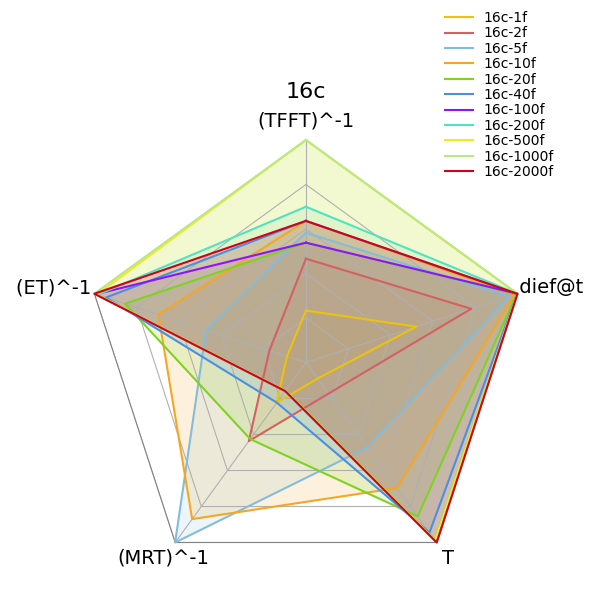
\includegraphics[scale=0.6]{../processed/NRT/small/checks/120-0.02/fixedcores/16c/plots/radar-dieft.png}
            \caption*{}
        \end{minipage}
    }

    \caption{Radial Plots for big stream: 120-0.02}
    \label{img:exps-read-input-variants}
\end{figure}


\paragraph{Radial plots - for a core number - different stream sizes\\}
\newpage

\begin{figure}[H]
    \centering
    % Temporarily adjust margins for wider content
    \makebox[\textwidth][c]{%
        \begin{minipage}{0.5\textwidth}
            \centering
            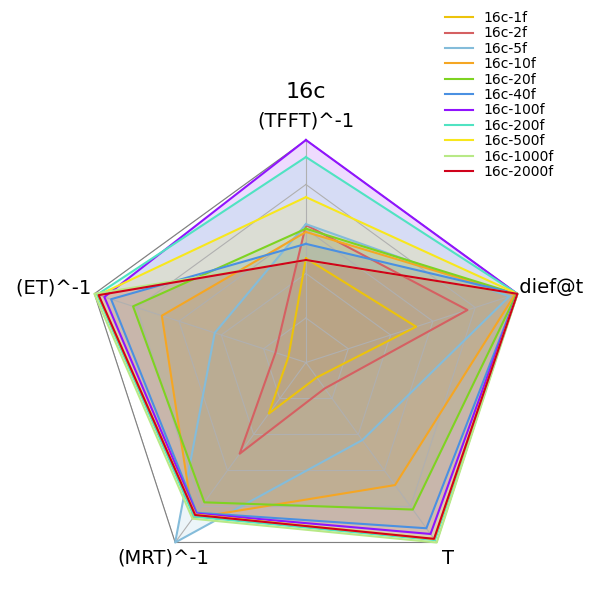
\includegraphics[scale=0.6]{../processed/NRT/small/checks/30-0.02/fixedcores/16c/plots/radar-dieft.png}
            \caption*{30-0.02}
        \end{minipage}
        \hspace{0.08\textwidth}
        \begin{minipage}{0.5\textwidth}
            \centering
            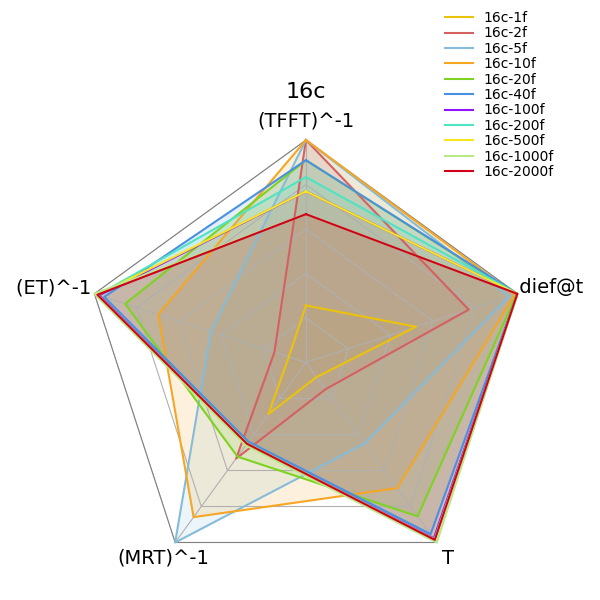
\includegraphics[scale=0.6]{../processed/NRT/small/checks/60-0.02/fixedcores/16c/plots/radar-dieft.png}
            \caption*{60-0.02}
        \end{minipage}
    }
    
    \vspace{0.5cm} % Vertical space between rows

    \makebox[\textwidth][c]{%
        \begin{minipage}{0.5\textwidth}
            \centering
            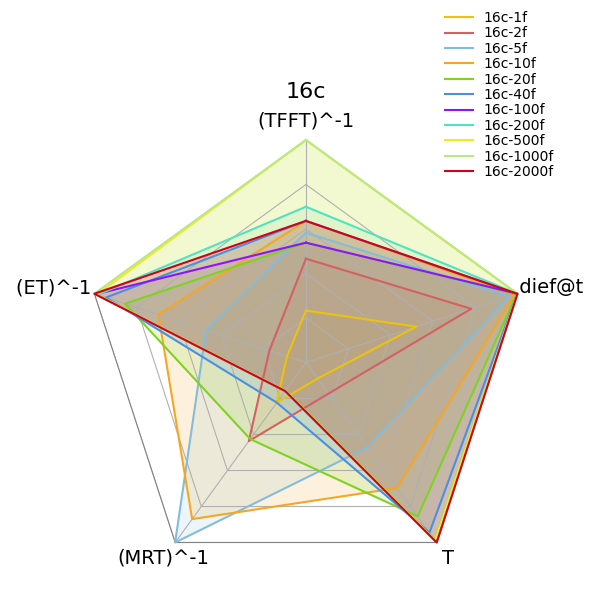
\includegraphics[scale=0.6]{../processed/NRT/small/checks/120-0.02/fixedcores/16c/plots/radar-dieft.png}
            \caption*{120-0.02}
        \end{minipage}
    }

    \caption{Radial Plots for 16c}
    \label{img:exps-read-input-variants}
\end{figure}

paragraph{MRT plots - for a core number 4c - different stream sizes\\}
\newpage

\begin{figure}[H]
    \centering
    % Temporarily adjust margins for wider content
    \makebox[\textwidth][c]{%
        \begin{minipage}{0.5\textwidth}
            \centering
            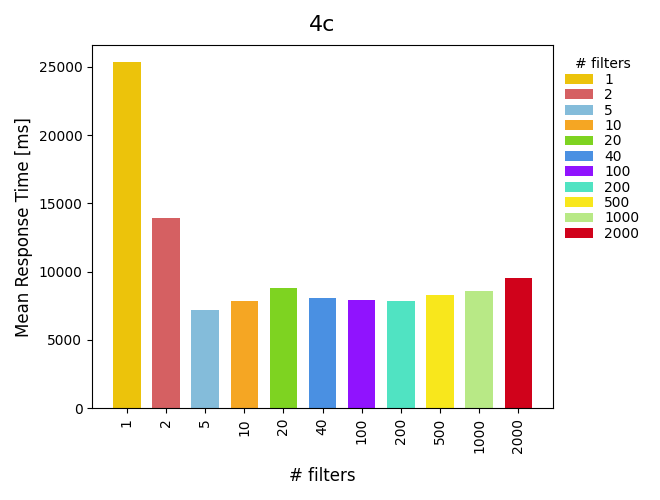
\includegraphics[scale=0.5]{../processed/NRT/small/checks/30-0.02/fixedcores/4c/plots/mrt.png}
            \caption*{30-0.02}
        \end{minipage}
        \hspace{0.1\textwidth}
        \begin{minipage}{0.5\textwidth}
            \centering
            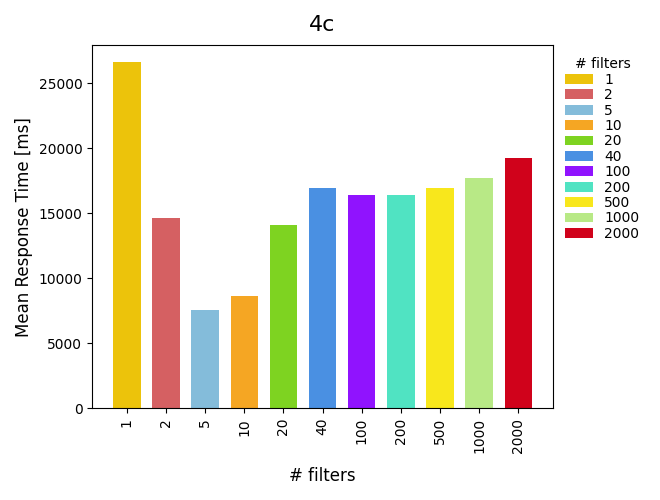
\includegraphics[scale=0.5]{../processed/NRT/small/checks/60-0.02/fixedcores/4c/plots/mrt.png}
            \caption*{60-0.02}
        \end{minipage}
    }
    
    \vspace{0.5cm} % Vertical space between rows

    \makebox[\textwidth][c]{%
        \begin{minipage}{0.5\textwidth}
            \centering
            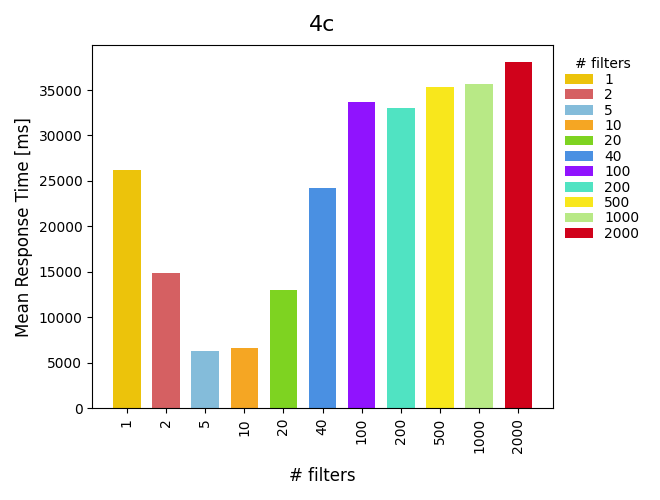
\includegraphics[scale=0.5]{../processed/NRT/small/checks/120-0.02/fixedcores/4c/plots/mrt.png}
            \caption*{120-0.02}
        \end{minipage}
    }

    \caption{MRT Plots for 4c}
    \label{img:exps-read-input-variants}
\end{figure}

\paragraph{Exec time plots - for a core number - different stream sizes\\}
\newpage
\begin{figure}[H]
    \centering
    % Temporarily adjust margins for wider content
    \makebox[\textwidth][c]{%
        \begin{minipage}{0.5\textwidth}
            \centering
            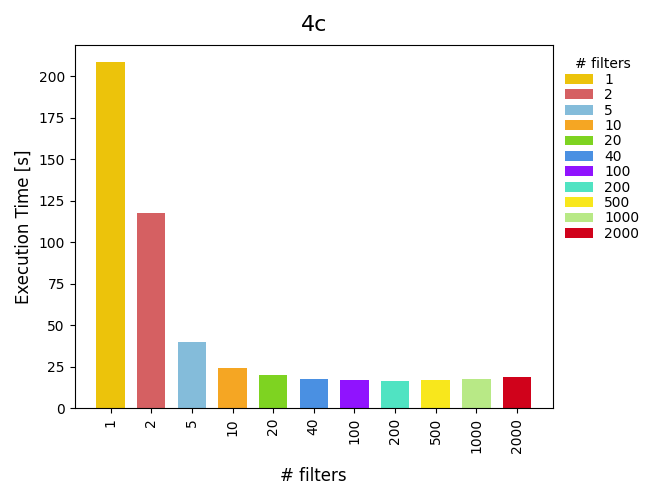
\includegraphics[scale=0.5]{../processed/NRT/small/checks/30-0.02/fixedcores/4c/plots/execTime.png}
            \caption*{30-0.02}
        \end{minipage}
        \hspace{0.1\textwidth}
        \begin{minipage}{0.5\textwidth}
            \centering
            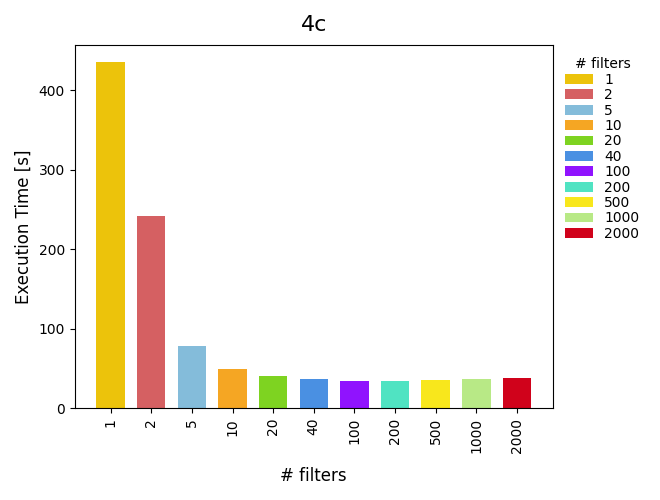
\includegraphics[scale=0.5]{../processed/NRT/small/checks/60-0.02/fixedcores/4c/plots/execTime.png}
            \caption*{60-0.02}
        \end{minipage}
    }
    
    \vspace{0.5cm} % Vertical space between rows

    \makebox[\textwidth][c]{%
        \begin{minipage}{0.5\textwidth}
            \centering
            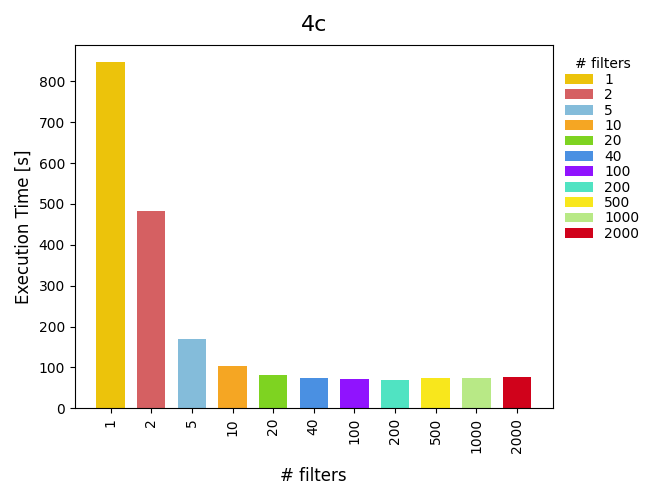
\includegraphics[scale=0.5]{../processed/NRT/small/checks/120-0.02/fixedcores/4c/plots/execTime.png}
            \caption*{120-0.02}
        \end{minipage}
    }

    \caption{Execution Time Plots for 4c}
    \label{img:exps-read-input-variants}
\end{figure}

\paragraph{MRT plots - for a core number 16 - different stream sizes\\}
\newpage

\begin{figure}[H]
    \centering
    % Temporarily adjust margins for wider content
    \makebox[\textwidth][c]{%
        \begin{minipage}{0.5\textwidth}
            \centering
            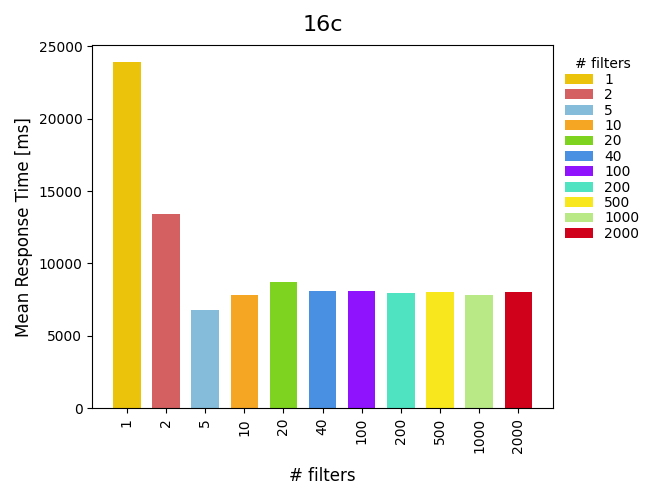
\includegraphics[scale=0.5]{../processed/NRT/small/checks/30-0.02/fixedcores/16c/plots/mrt.png}
            \caption*{30-0.02}
        \end{minipage}
        \hspace{0.1\textwidth}
        \begin{minipage}{0.5\textwidth}
            \centering
            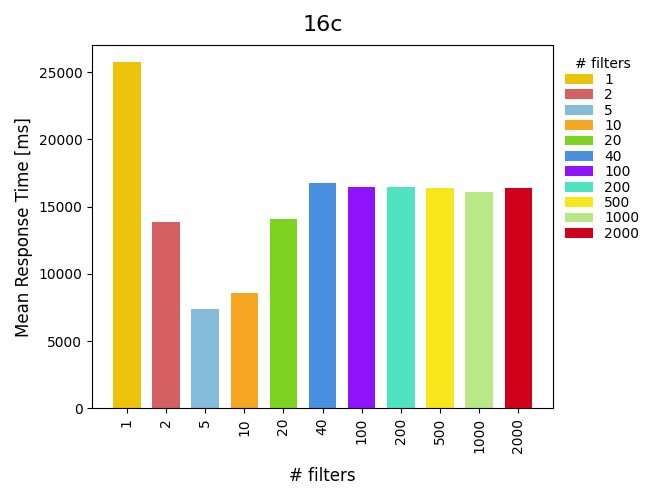
\includegraphics[scale=0.5]{../processed/NRT/small/checks/60-0.02/fixedcores/16c/plots/mrt.png}
            \caption*{60-0.02}
        \end{minipage}
    }
    
    \vspace{0.5cm} % Vertical space between rows

    \makebox[\textwidth][c]{%
        \begin{minipage}{0.5\textwidth}
            \centering
            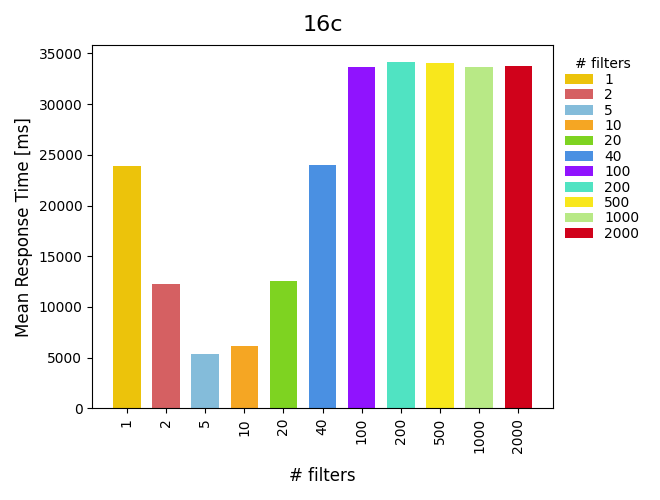
\includegraphics[scale=0.5]{../processed/NRT/small/checks/120-0.02/fixedcores/16c/plots/mrt.png}
            \caption*{120-0.02}
        \end{minipage}
    }

    \caption{MRT Plots for 16c}
    \label{img:exps-read-input-variants}
\end{figure}

\paragraph{Exec time plots - for a core number - different stream sizes\\}
\newpage
\begin{figure}[H]
    \centering
    % Temporarily adjust margins for wider content
    \makebox[\textwidth][c]{%
        \begin{minipage}{0.5\textwidth}
            \centering
            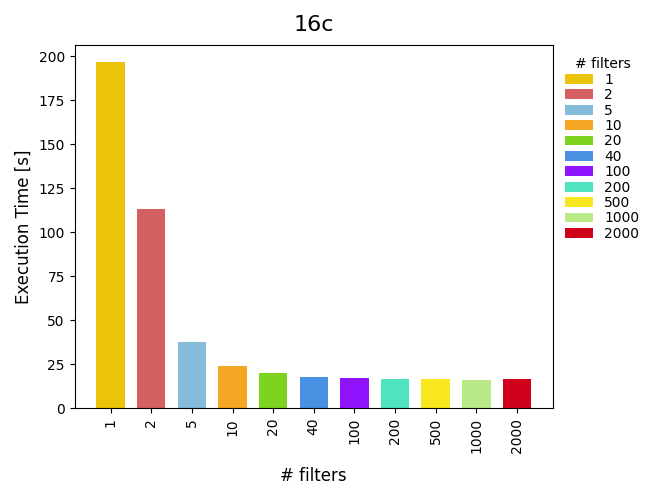
\includegraphics[scale=0.5]{../processed/NRT/small/checks/30-0.02/fixedcores/16c/plots/execTime.png}
            \caption*{30-0.02}
        \end{minipage}
        \hspace{0.1\textwidth}
        \begin{minipage}{0.5\textwidth}
            \centering
            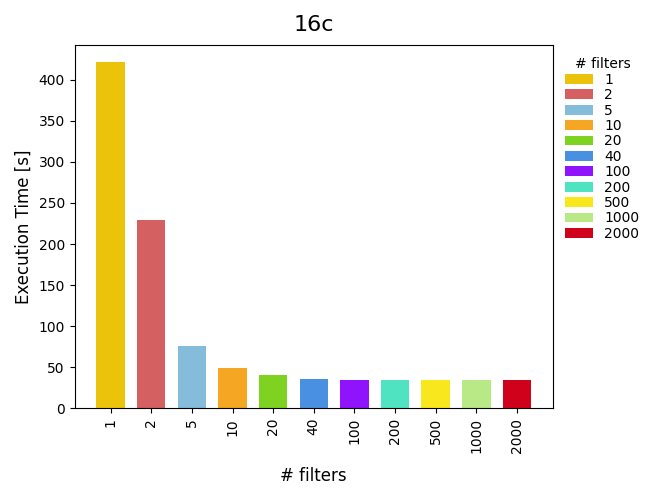
\includegraphics[scale=0.5]{../processed/NRT/small/checks/60-0.02/fixedcores/16c/plots/execTime.png}
            \caption*{60-0.02}
        \end{minipage}
    }
    
    \vspace{0.5cm} % Vertical space between rows

    \makebox[\textwidth][c]{%
        \begin{minipage}{0.5\textwidth}
            \centering
            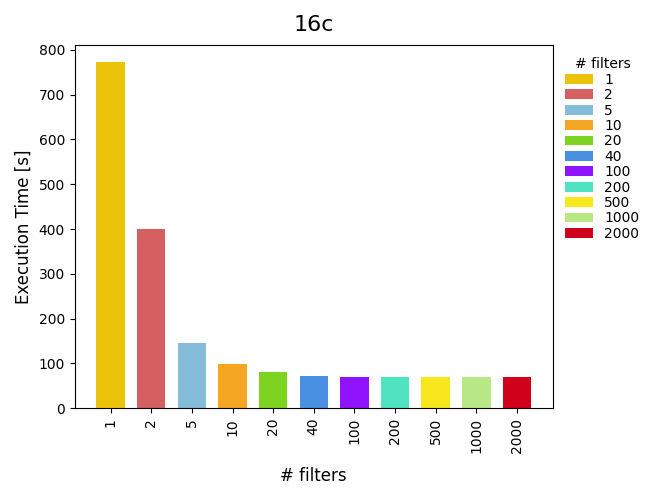
\includegraphics[scale=0.5]{../processed/NRT/small/checks/120-0.02/fixedcores/16c/plots/execTime.png}
            \caption*{120-0.02}
        \end{minipage}
    }

    \caption{Execution Time Plots for 16c}
    \label{img:exps-read-input-variants}
\end{figure}

\paragraph{Trace and response time trace for 16c and big stream\\}
\newpage

\begin{figure}[H]
    \centering
    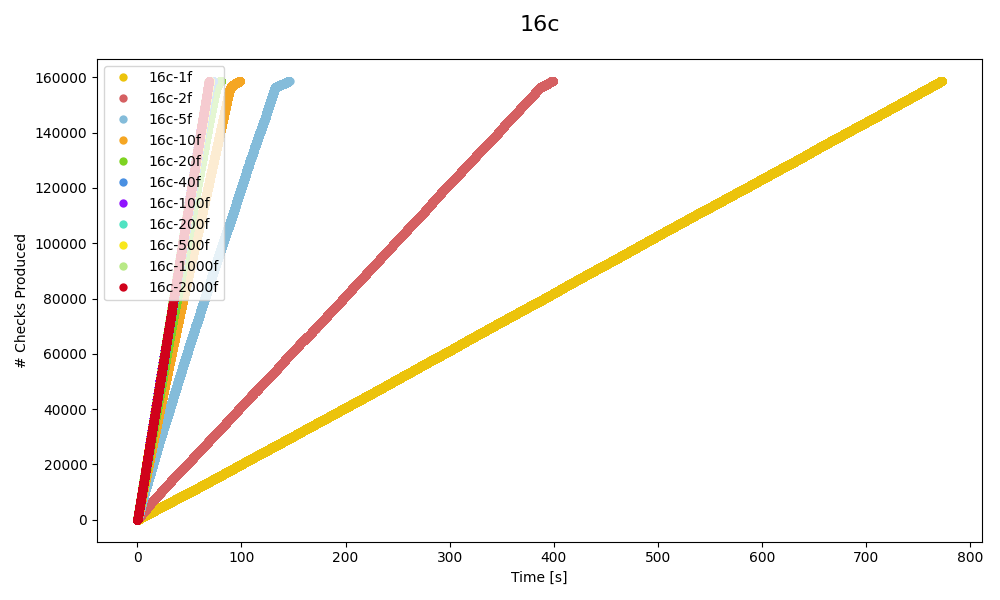
\includegraphics[scale=0.5]{../processed/NRT/small/checks/120-0.02/fixedcores/16c/plots/traces.png}
    \caption*{Trace}
\end{figure}

\begin{figure}[H]
    \centering
    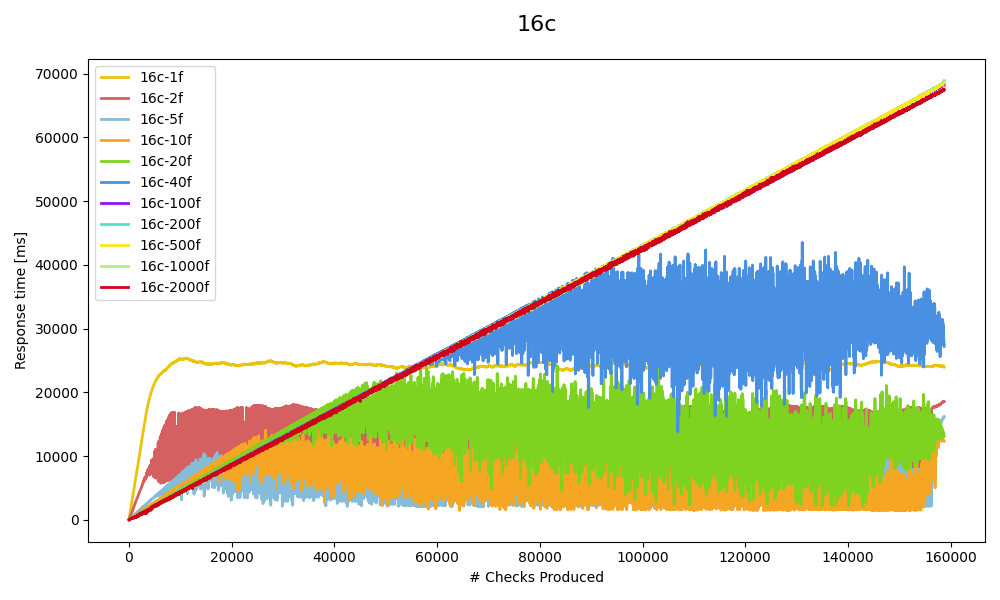
\includegraphics[scale=0.5]{../processed/NRT/small/checks/120-0.02/fixedcores/16c/plots/traces-response-time-reduced.png}
    \caption*{Trace Response Time reduced}
\end{figure}


2. Show how incrementing the resources (number of cores) help to improve the behavior


\begin{figure}[H]
    \centering
    % Temporarily adjust margins for wider content
    \makebox[\textwidth][c]{%
        \begin{minipage}{0.5\textwidth}
            \centering
            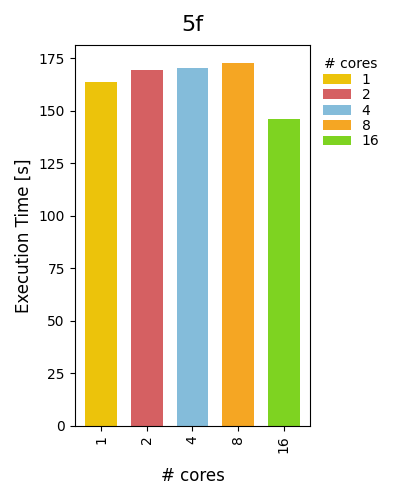
\includegraphics[scale=0.6]{../processed/NRT/small/checks/120-0.02/fixedfilters/5f/plots/execTime.png}
            \caption*{}
        \end{minipage}
        \hspace{0.08\textwidth}
        \begin{minipage}{0.5\textwidth}
            \centering
            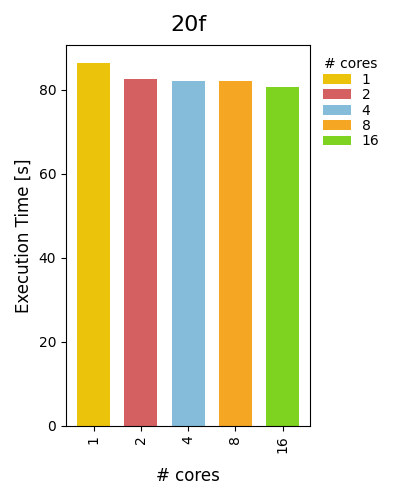
\includegraphics[scale=0.6]{../processed/NRT/small/checks/120-0.02/fixedfilters/20f/plots/execTime.png}
            \caption*{}
        \end{minipage}
    }
    
    \vspace{0.5cm} % Vertical space between rows

    \makebox[\textwidth][c]{%
        \begin{minipage}{0.5\textwidth}
            \centering
            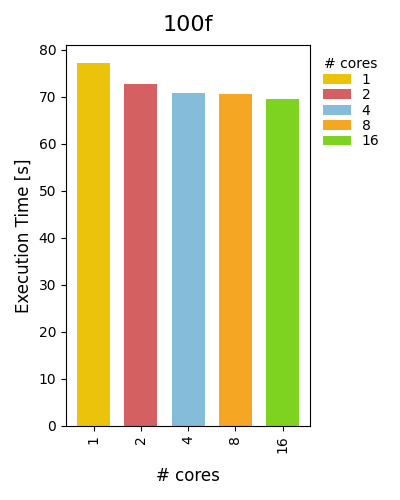
\includegraphics[scale=0.6]{../processed/NRT/small/checks/120-0.02/fixedfilters/100f/plots/execTime.png}
            \caption*{}
        \end{minipage}
        \hspace{0.08\textwidth}
        \begin{minipage}{0.5\textwidth}
            \centering
            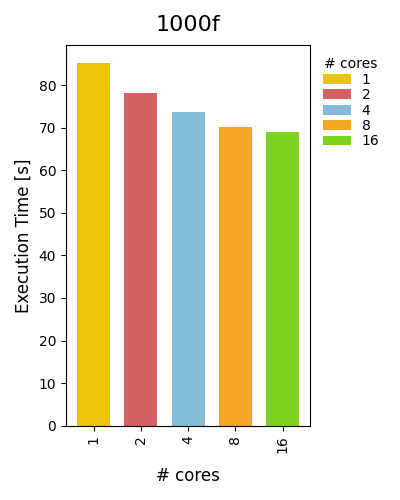
\includegraphics[scale=0.6]{../processed/NRT/small/checks/120-0.02/fixedfilters/1000f/plots/execTime.png}
            \caption*{}
        \end{minipage}
    }

    \caption{Radial Plots for big stream: 120-0.02}
    \label{img:exps-read-input-variants}
\end{figure}


Ideas on the analysis so far:

\begin{itemize}
    \item More cores help to improve the behavior, especially for the variants with large number of filters (expected).
    \item For a same core configuration (e.g. 16 cores), the total execution time (time to process all the stream input) is larger for the approaches with less cores, tending to decrease. However the continuous behavior is different: the best is observed for a number of filters in the range of 5-10 filters. From that point and on the continuous behavior tends to degrade when increasing the number filters, especially for bigger stream sizes. Even larger than the lowest number of filters version (close to a sequential version) in these cases. This can be due to an overhead on the number of goroutines utilized and the overhead in the communication of the pipeline that this is causing.
\end{itemize}


These same conclusions are easily to observe in:

\begin{figure}[H]
    \centering
    % Temporarily adjust margins for wider content
    \hspace*{-3cm} % Move content to the left by 2 cm (adjust as needed)
    \begin{minipage}{0.5\textwidth}
        \centering
        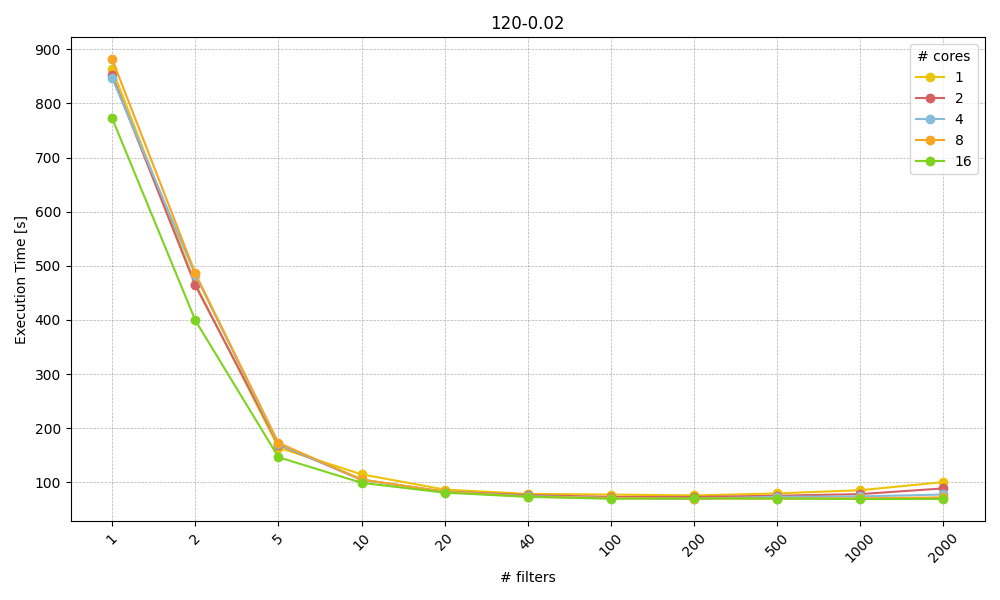
\includegraphics[scale=0.4]{../processed/NRT/small/checks/120-0.02/combined/execTime-1.png}
        \caption*{}
    \end{minipage}
    \hspace{0.16\textwidth}
    \begin{minipage}{0.5\textwidth}
        \centering
        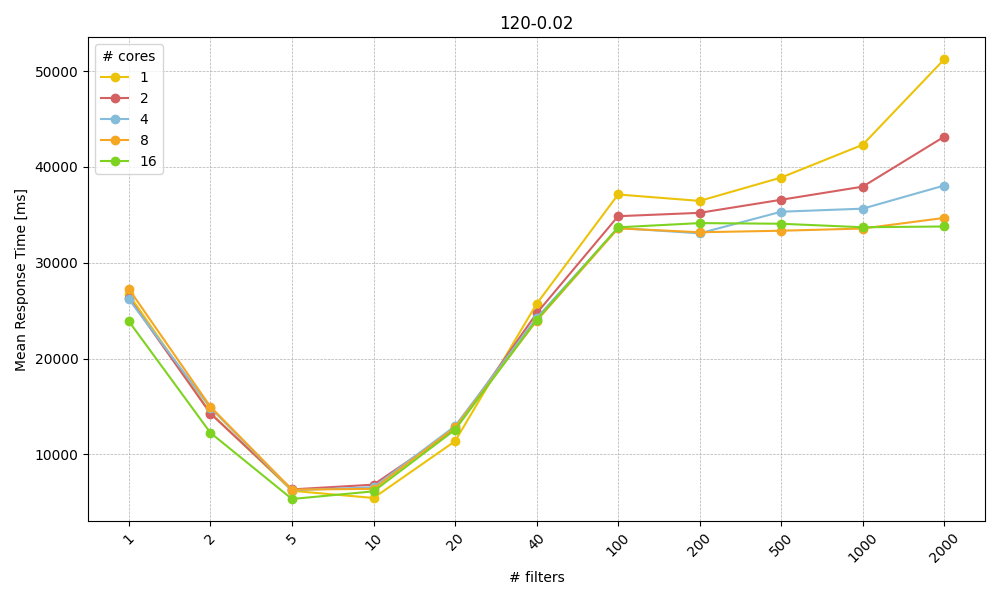
\includegraphics[scale=0.4]{../processed/NRT/small/checks/120-0.02/combined/mrt-1.png}
        \caption*{}
    \end{minipage}
    
    \vspace{0.5cm} % Vertical space between rows

    \hspace*{-3cm} % Move content to the left for the second row
    \begin{minipage}{0.5\textwidth}
        \centering
        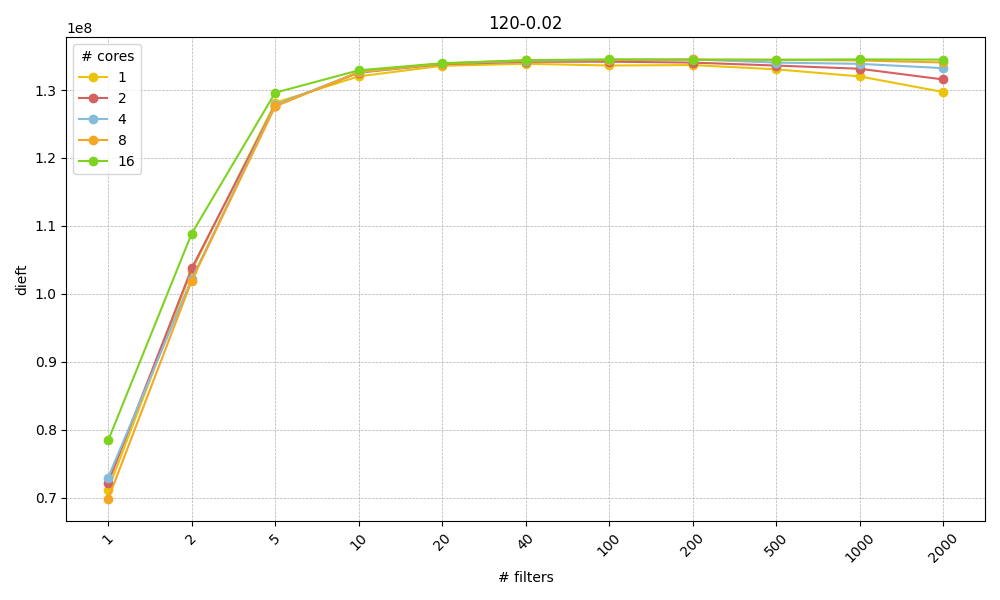
\includegraphics[scale=0.4]{../processed/NRT/small/checks/120-0.02/combined/dieft-1.png}
        \caption*{}
    \end{minipage}
    \hspace{0.16\textwidth}
    \begin{minipage}{0.5\textwidth}
        \centering
        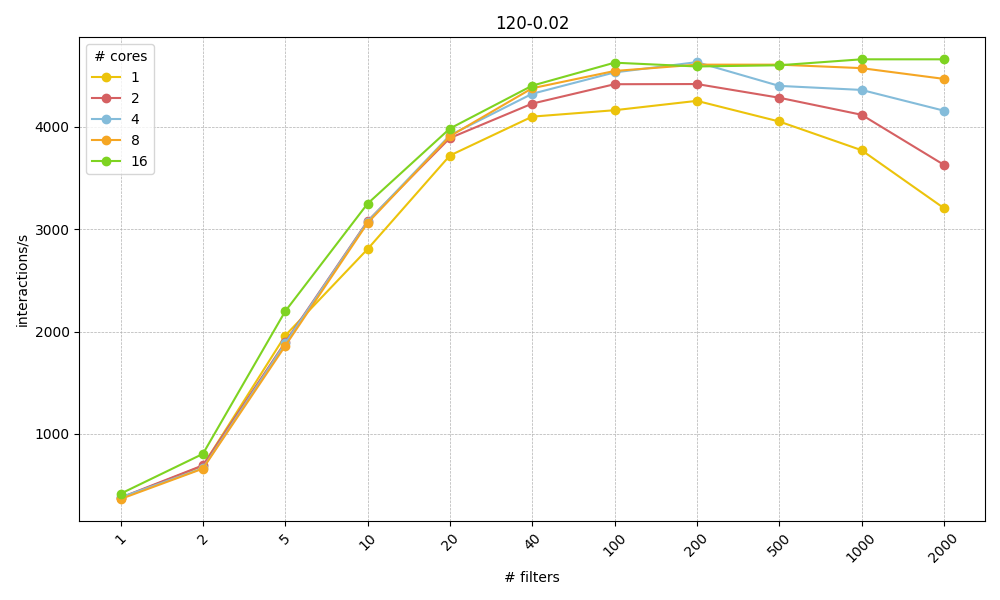
\includegraphics[scale=0.4]{../processed/NRT/small/checks/120-0.02/combined/interactions-1.png}
        \caption*{}
    \end{minipage}

    \caption{Radial Plots for big stream: 120-0.02}
    \label{img:exps-read-input-variants}
\end{figure}

\textcolor{red}{La pregunta es, por qué teniendo menor tiempo de ejecución, el mrt es superior? - Dar una explicación a esto...}

\subsubsection{Differences among the different stream sizes}

\section{Experiments Summary}


\subsection{E1 - NRT}

\textbf{ONLY CHECKS in these experiments}

Bank Sizes:
\begin{itemize}
    \item Small: $|Card| = 2000$, $|ATM| = 50$
    \item Medium: $|Card| = 500000$,  $|ATM| = 1000$
\end{itemize}

Stream Sizes:


\begin{table}[H]
    \begin{tabular}{|c|c|c|c|c|c|}
    \hline
    Bank Size & Num Days & Anomalous Ratio & Stream Size & Regular tx & Anomalous tx \\ \hline
    Small     & 30       & $0.02\ (2\%)$   & 39959       & 39508      & 451 $1\%$    \\ \hline
    Small     & 60       & $0.02\ (2\%)$   & 80744       & 79005      & 1739         \\ \hline
    Small     & 120      & $0.02\ (2\%)$   & 160750      & 157756     & 2994         \\ \hline
    Medium    & 7        & $0.03\ (3\%)$   & 2428286     &            &              \\ \hline
    Medium    & 15       & $0.03\ (3\%)$   & 4856573     & 4805920    & 50653        \\ \hline
    Medium    &          &                 &             &            &              \\ \hline
    Big       &          &                 &             &            &              \\ \hline
    Big       &          &                 &             &            &              \\ \hline
    Big       &          &                 &             &            &              \\ \hline
    \end{tabular}
\end{table}
    
    
For different core variations, we are going to try different combinations of the system in terms
of the number of the maximum number of cards per filter, that consequently will produce an inverse variation in the number of filters of the system.

\subsubsection{Small Bank Size}
    
\begin{table}[H]
    \renewcommand{\arraystretch}{1.5} % control row height
    \centering
    \begin{tabular}{|c|c|}
    \hline
    \# cards per filter & \# filters \\ \hline
    2000   &   1     \\ \hline
    1000   &   2     \\ \hline
    400 &   5     \\ \hline
    200  &   10     \\ \hline
    100 &   20    \\ \hline
    50  &   40    \\ \hline
    20  &   100    \\ \hline
    10  &   200    \\ \hline
    4  &   500    \\ \hline
    2  &   1000    \\ \hline
    1  &   2000    \\ \hline
    \end{tabular}
\end{table}
    
\begin{itemize}
    \item \# of times / runs each job $=10$.
    \item Maximum RAM limited to 16GB.
    \item Run for 1c, 2c, 4c, 8c and 16c.
\end{itemize}
  
\subsubsection{Medium Bank Size}
  
\textcolor{red}{For these experiments, to generate the stream of tx, we needed to simplify this process in order to be able to generate a stream in a feasible amount of time. In particular we used the simplifed version of the \texttt{txGenerator.py}: \texttt{txGenerator-simplified.py} $\rightarrow$ with a random ATM-subset instead of a closest to client ATM-subset. Also variation on the transaction distribution times.}
  

- Initial filter configuration setups:
\begin{table}[H]
\renewcommand{\arraystretch}{1.5} % control row height
\centering
\begin{tabular}{|c|c|}
\hline
\# cards per filter & \# filters \\ \hline
500000   &   1     \\ \hline
100000   &   5     \\ \hline
50000 &   10     \\ \hline
5000  &   100     \\ \hline
2000 &   250    \\ \hline
1000  &   500    \\ \hline
500  &   1000    \\ \hline
250  &   2000    \\ \hline
100  &   5000    \\ \hline
50  &   10000    \\ \hline
10  &   50000    \\ \hline
\end{tabular}
\end{table}

Run with:
\begin{itemize}
    \item 16GB RAM
    \item x1 run each job
\end{itemize}

\begin{itemize}
    \item x: Run and plots done.
    \item " ": Not run.
    \item outMem: out of memory error.
\end{itemize}

\textbf{Stream - 7 Days}
\begin{table}[H]
  \begin{tabular}{|c|c|c|c|c|c|c|c|c|c|c|c|}
  \hline
  \#cores & 1f & 5f & 10f & 100f & 250f & 500f & 1000f & 2000f & 5000f & 10000f & 50000f \\ \hline
  1       &   & x & x & x & x & x & x & x & x & x &        \\ \hline
  2       &   & x & x & x & x & x & x & x & x & x &        \\ \hline
  4       &   & x & x & x & x & x & x & x & x & x &        \\ \hline
  8       &   & x & x & x & x & x & x & x & x & x &        \\ \hline
  16      & x & x & x & x & x & x & x & x & x & x & outMem \\ \hline
  \end{tabular}
\end{table}

Plots:
\begin{itemize}
    \item FixedCores: OK
    \item FixedFilters: OK
    \item Combined: TODO, increase RAM memory to do it, higher than 64GB...
\end{itemize}



\textbf{Stream - 15 Days}
\begin{table}[H]
  \begin{tabular}{|c|c|c|c|c|c|c|c|c|c|c|c|}
  \hline
  \#cores & 1f & 5f & 10f & 100f & 250f & 500f & 1000f & 2000f & 5000f & 10000f & 50000f \\ \hline
  1       &   & x & x & x & x & x & x & x & x & x &        \\ \hline
  2       &   & x & x & x & x & x & x & x & x & x &        \\ \hline
  4       &   & x & x & x & x & x & x & x & x & x &       \\ \hline
  8       & x & x & x & x & x & x & x & x & x & x &        \\ \hline
  16      & x & x & x & x & x & x & x & x & x & x & outMem \\ \hline
  \end{tabular}
\end{table}

Plots:
$\rightarrow$ Not done so far, only the reduced version explained next. Since for the 7D plots
we could already observe that a large number of filters did not produce any advantage, we prefer
to reduce the interval of filters in which to show the plots.
\begin{itemize}
    \item FixedCores: TODO
    \item FixedFilters: TODO
    \item Combined: TODO
\end{itemize}
  

Based on the results seen (it seems that a really great number of filters is not beneficial), we want to see what happens with a combination of a lower number of filters (like in the experiments for the small bank database):


\begin{table}[H]
    \renewcommand{\arraystretch}{1.5} % control row height
    \centering
    \begin{tabular}{|c|c|}
    \hline
    \# cards per filter & \# filters \\ \hline
    2000   &   1     \\ \hline
    1000   &   2     \\ \hline
    400 &   5     \\ \hline
    200  &   10     \\ \hline
    100 &   20    \\ \hline
    50  &   40    \\ \hline
    20  &   100    \\ \hline
    10  &   200    \\ \hline
    4  &   500    \\ \hline
    2  &   1000    \\ \hline
    1  &   2000    \\ \hline
    \end{tabular}
\end{table}


\textbf{Stream - 7 Days}
\begin{table}[]
    \begin{tabular}{|c|c|c|c|}
    \hline
    \#cores & 20f & 40f & 200f \\ \hline
    1       &     &     &      \\ \hline
    2       &     &     &      \\ \hline
    4       &     &     &      \\ \hline
    8       &     &     &      \\ \hline
    16      &     &     &      \\ \hline
    \end{tabular}
\end{table}

Results: DONE

Plots:
\begin{itemize}
    \item FixedCores: Done
    \item FixedFilters: Done
    \item Combined: TODO, increase RAM memory to do it, higher than 64GB...
\end{itemize}


\textbf{Stream - 15 Days}
\begin{table}[]
    \begin{tabular}{|c|c|c|c|c|}
    \hline
    \#cores & 2f & 20f & 40f & 200f \\ \hline
    1       &    &     &     &      \\ \hline
    2       &    &     &     &      \\ \hline
    4       &    &     &     &      \\ \hline
    8       &    &     &     &      \\ \hline
    16      &    &     &     &      \\ \hline
    \end{tabular}
\end{table}

Results: Done

Plots:
\begin{itemize}
    \item FixedCores: Obtaining
    \item FixedFilters: TODO $\rightarrow$ not for the moment
    \item Combined: TODO, increase RAM memory to do it, higher than 64GB... $\rightarrow$ not for the moment
\end{itemize}


\subsection{NEW: Reduced comparison}

Plots for the medium gdb, with a reduced number of filters (1f...200f) and including the baseline, to see better what happens.

Obtaining baselines run
\begin{itemize}
    \item 7D: 1c, 2c, 4c, 8c, 16c
    \item 15D: 1c, 2c, 4c, 8c, 16c
\end{itemize}

Obtaining plots - only fixed cores plots
\begin{itemize}
    \item 7D: 
    \item 15D: 
\end{itemize}

\end{document}